%---------- Quarto Capitulo ----------
\chapter{Ferramentas de desenvolvimento}
Algumas das organizações existentes que desenvolvem estes dispositivos, como por exemplo, a Google, a Apple e Microsoft, cada uma com sua plataforma, Android, iOS e Windows, respectivamente, oferecem aos desenvolvedores ferramentas e ambientes de desenvolvimento ricos em bibliotecas que fornecem suporte e facilidades no desenvolvimento de aplicativos.

\begin{figure}[h]
	\center
	\subfigure[fig:androidstudio][Android Studio]{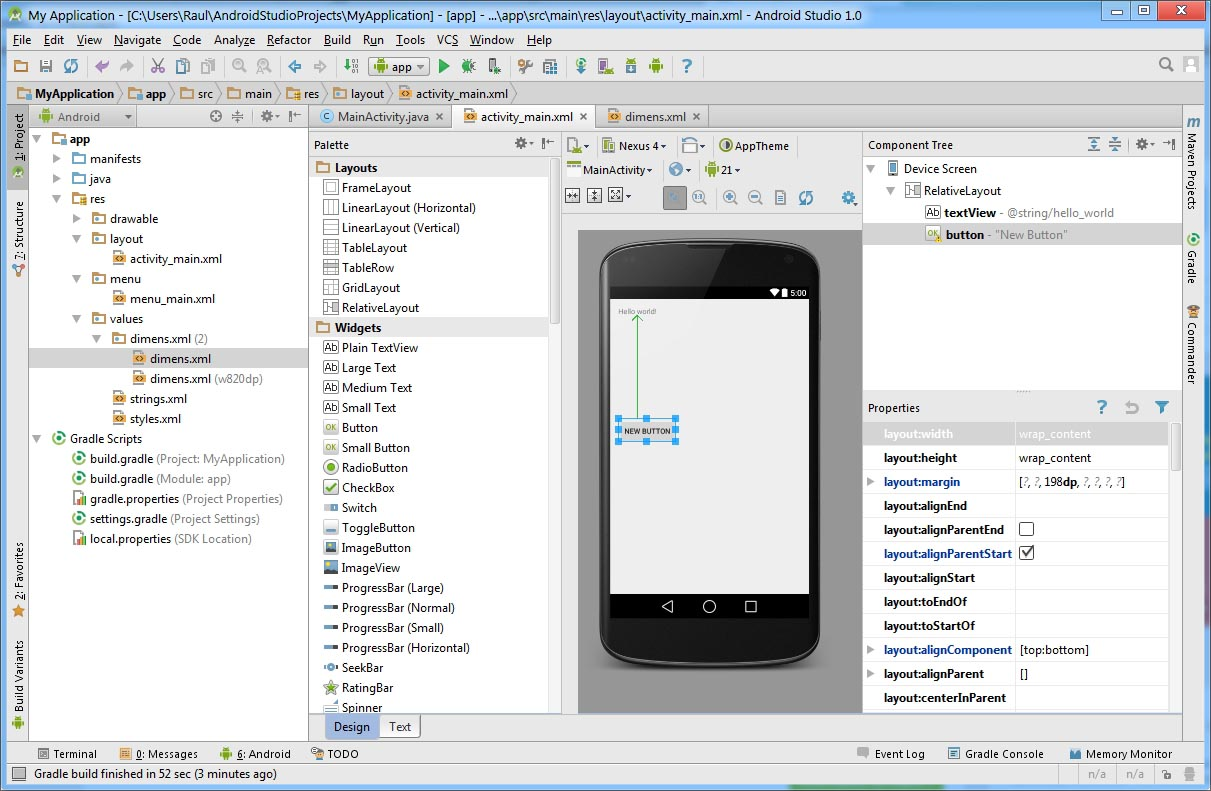
\includegraphics[width=7cm]{androidstudio.jpg}}
	\qquad
	\subfigure[fig:xcode][XCode]{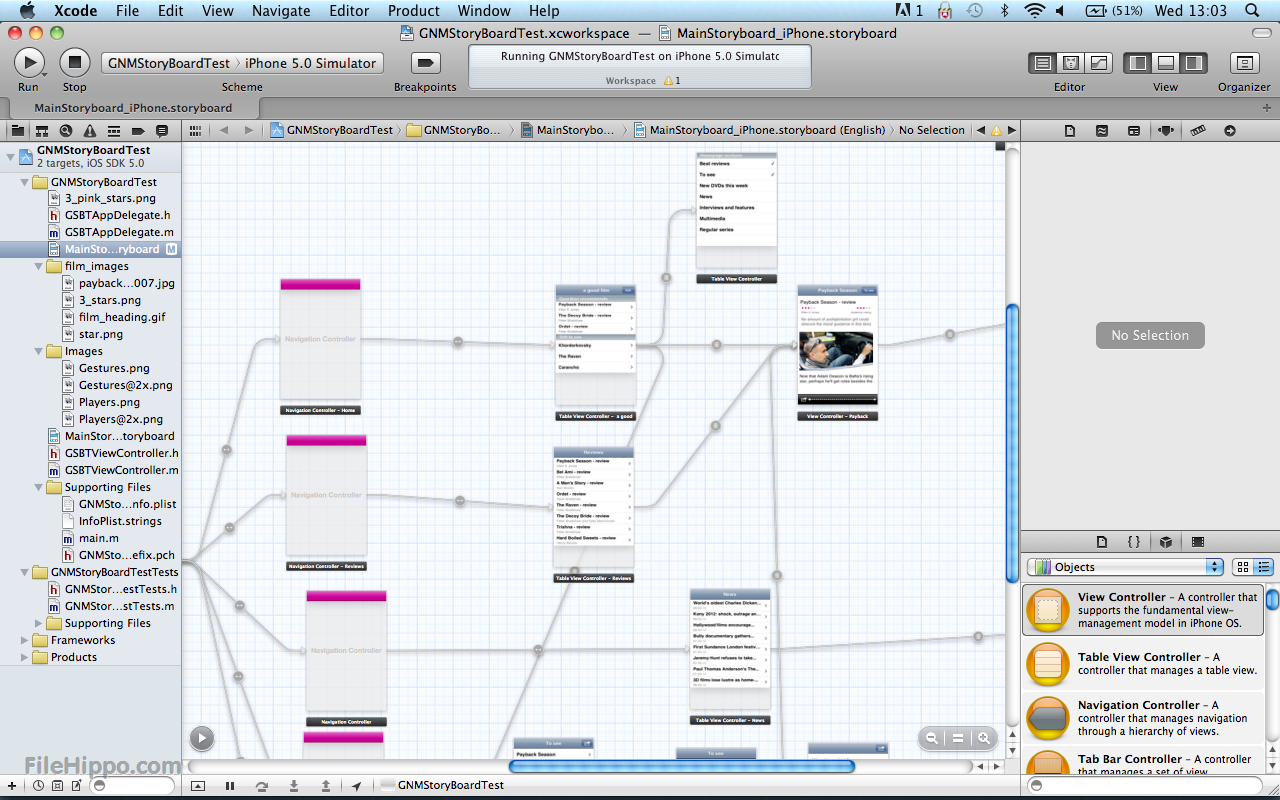
\includegraphics[width=7.5cm]{xcode.png}}
	\qquad
	\subfigure[fig:visualstudio][Visual Studio]{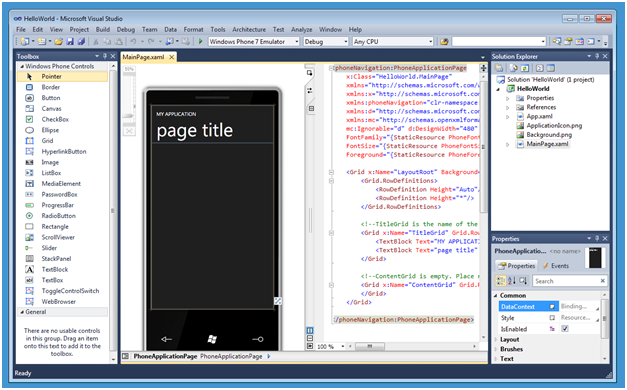
\includegraphics[width=7.3cm]{visualstudio.png}}
	\caption{SDKs oferecidos pelas empresas (a)Google, (b)Apple e (c)Microsoft}
\end{figure}

Essas empresas também mantêm sites voltados aos desenvolvedores com documentos e informações sobre como utilizar as bibliotecas e as ferramentas para o desenvolvimento de aplicativos.

\section{Linguagens de Programação e Frameworks de Desenvolvimento}
Além dos \sigla{SDKs}{Software Development Kit}, desses ambientes de desenvolvimento disponibilizados por essas empresas, outras organizações também desenvolvem tecnologias que apoiam a criação de aplicativos para essas platafomas como por exemplo as empresas Appcelerator e Apache. A Appcelerator disponibiliza um ambiente de desenvolvimento completo com IDE, plugins e bibliotecas conhecido como Titanium IDE, já a Apache disponibiliza ao desenvolvedores uma plataforma para criar aplicativos utilizando as tecnologias Javascript, HTML e CSS chamada Cordova.

Várias outras organizações utilizam o Apache Cordova como núcleo em seus frameworks para o desenvolvimento de aplicativos para dispositivo móveis, como é o caso do Adobe PhoneGap, Intel XDK e Ionic Framework.

\begin{figure}[!htb]
	\centering
	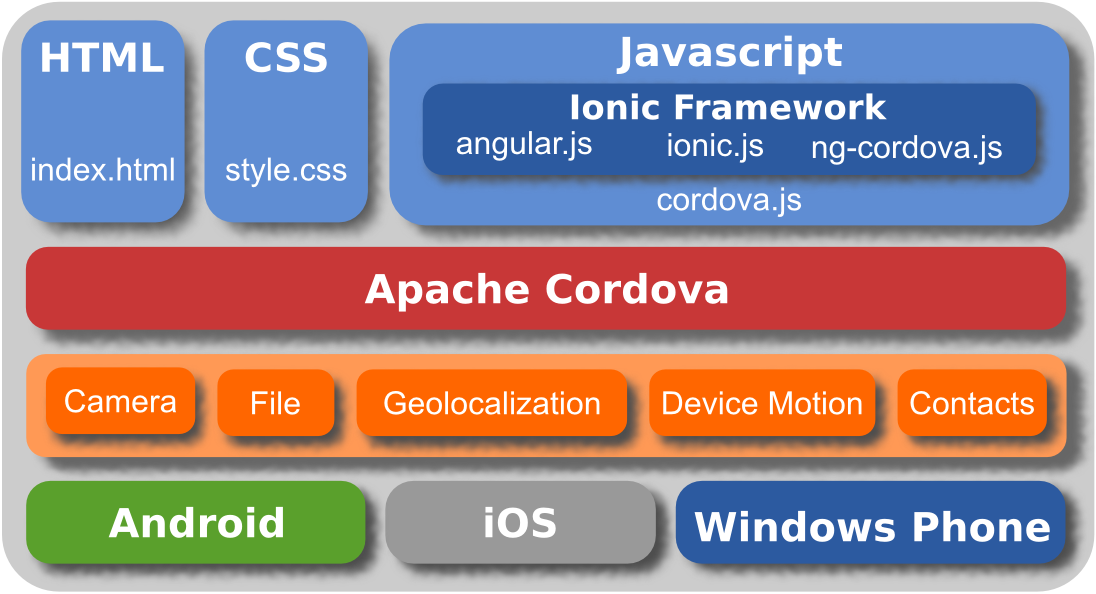
\includegraphics[width=.7\textwidth]{ionicarch.png} % <- formatos PNG, JPG e PDF
	\caption[Arquitetura do Ionic framework]{Arquitetura do Ionic framework}
	\label{fig:ionicarch}
\end{figure}

A implementação do aplicativo para dispositivo móvel utilizou o Ionic Framework. Como ele utiliza o Apache Cordova, a aplicação foi desenvolvida com o uso das Linguagens Javascript, HTMLe CSS.

\begin{figure}[!htb]
	\centering
	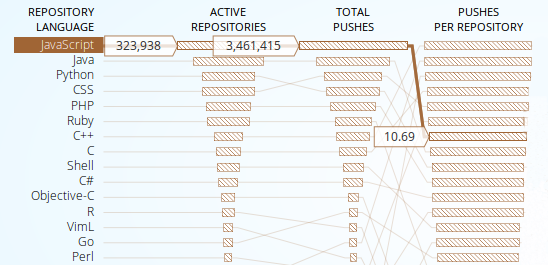
\includegraphics[width=1.1\textwidth]{javascript-st.png} % <- formatos PNG, JPG e PDF
	\caption[Linguagens com maior número de repositórios ativos no GitHub]{Gráfico sobre as linguagens com repositórios ativos no GitHub}
	\label{fig:javascript}
\end{figure}

Javascript é a linguagem com o maior número de repositórios ativos no GitHub. Com esse grande número de repositórios, a linguagem Javascript se torna uma opção muito atrativa na escolha como linguagem principal no desenvolvimento de aplicativos, pois existem muitas pessoas utilizando a linguagem e isso faz com que seja fácil de encontrar exemplos de uso de código, existe a facilidade na obtenção de respostas de dúvidas em foruns de discussão, e também acontece o aumento na quantidade de bibliotecas utéis que podem ser utilizadas em diversos tipos de projetos.

Javascript está se tornando muito popular também como linguagem de backend, com o Node.Js.
\begin{citacao}
Como um framework assíncrono dirigido a eventos, Node.js foi desenhado para contruir aplicações de rede escaláveis. No exemplo a seguir, muitas conexões podem ser manipuladas concorrentemente. A cada conexão uma chamada é disparada, mas se nenhuma requisição é feita o Node dorme. \cite{nodejs}

\begin{verbatim}
  const http = require('http');
  const hostname = '127.0.0.1';
  const port = 1337;

  http.createServer((req, res) => {
    res.writeHead(200, { 'Content-Type': 'text/plain' });
    res.end('Hello World\n');
  }).listen(port, hostname, () => {
    console.log(`Running at http://${hostname}:${port}/`);
  });
\end{verbatim}
\end{citacao}

O Javascript pode ser encontrado até como linguagem auxiliar para manipulação de dados em Banco de Dados, como é o caso do MongoDB, um banco de dados orientado a documentos que utiliza o \sigla{JSON}{JavaScript Object Notation} como estrutura de dados.
\begin{citacao}
MongoDB faz com que trabalhar com banco de dados seja simples e elegante. Ele utiliza um modelo de dados JSON que é mapeado para a sua aplicação, e possui esquemas dinâmicos que permitem uma iteração muito rápida. Tem bibliotecas para a linguagem que você utiliza para codificar. E ele tem uma linguagem de consulta expressiva que lhe permite buscar, ordenar, agregar dados sem a necessidade de escrever código extra. Ele ainda é mais fácil de implantar, provisionar e escalar.\cite{mongodb}
\end{citacao}